\chapter{Introduction}\label{chap:introduction}
Indoor environments pose various challenges for localization and mapping algorithms, mainly because many unique settings exist.
Finding a solution which works for a lot of setups is therefore rather difficult. \newline
Let's start by giving an example for a typical indoor localization and mapping problem and then move on to describe the common problem on a higher level.\newline
Sometimes, finding your smartphone at home might be harder than you think, especially if you have no clue where you left it.
If nothing helps you will probably ask a family member, room mate or partner to help you out with a phone call.
Once you hear the sound of your exotic ring tone you will most likely start following it until you find your phone. \newline
This might sound like a silly example but in fact it covers the basic elements of a localization problem: A set of receivers (ears), an environment (house or apartment) and the unknown location of a source (smartphone).\newline
J. Bordoy et al. proposed a solution for almost the same problem \cite{bordoy2019exploiting}. 
They used a combination of direct path and reflected ultrasound signals. 
Former is usually referred to as line-of-sight (LOS) and latter as non-light-of-sight (NLOS) scenario.
LOS describes the case where a localization system is able to "see" the source to be located and NLOS is the case where an object/obstacle is blocking the direct path between the localization system and the source.\newline
Let's move on to an indoor mapping/imaging example from Flávio Ribeiro et al. where they try to estimate the geometry of a room with compact microphone arrays \cite{ribeiro2011geometrically}. 
The source, in this case a loudspeaker, is co-located with the receiver array. 
A known test signal is emitted through the source and the reflections of the test signal are used to estimate the room geometry. 
Since they apply directional constraints on the received signal, they are able to extract the relevant reflections and therefore estimate the dimensions of the room.\newline
Even though both of these proposals are trying to solve two completely different problems, they share a common "interface" to the physical world. 
This interface is illustrated in \figref{fig:Intro}.

\begin{figure}[H]
    \begin{center}
    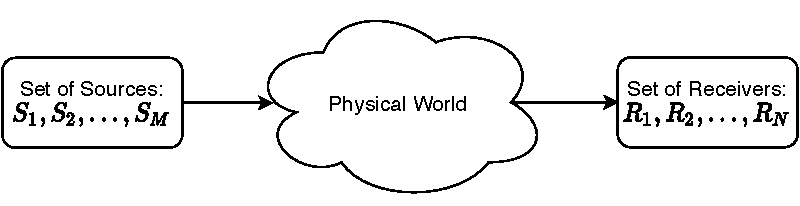
\includegraphics[width=\textwidth]{figures/introduction/figIntro.pdf}
    \end{center}
    \caption[Problem Generalization]{Problem Generalization}
    \label{fig:Intro}
\end{figure}

The sources emit a signal through the room and interact with the environment. 
Effects like path attenuation, reflections, scattering and diffraction will modify the signal as it propagates through the room \cite{vorlander2013computer}.
The result of these effects is perceived and recorded by the receivers.
Modelling and simulating the sources, receivers, the environment, the effects and the receivers will enable creating test data for the problems like \cite{bordoy2019exploiting} and \cite{ribeiro2011geometrically}.
Tests can be performed and evaluated in virtual environments and setups.
Creating a tool which allows us to do these things is therefore very useful.
The question is, how can this be achieved?

One very promising answer to this question is Acoustic/Ultrasonic Ray Tracing.
The hearing range of humans is $20\text{Hz} < f < 20 \text{kHz}$ and will be called "audible spectrum".
For frequencies higher than $20\text{kHz}$ we enter the ultrasound spectrum.
A lot of the general acoustic laws for the audible spectrum apply for the ultrasound spectrum as well.
There are however two main differences which are very important when designing an indoor localization or mapping system:\newline
1. Imagine having a system which depends on audible sound waves.
If the system is to be used in a human inhabited indoor environment, the system could be very annoying to people, especially for periodic sources.
This statement however is purely subjective and based on reasonable common sense.
Nonetheless it is a practical reason not to use frequencies below 20kHz.\newline
2. The second reason is that ultrasound waves can be approximated by rays, because of their reflection behavior.
This is mainly due to the fact that the relation between wavelength and the size of a reflecting surface is important.
For 20kHz the wavelength is approximately 17mm and for 100kHz it's approximately 3.4mm.
If the surface is much larger than the wavelength, which is the case for a lot of objects and obstacles, it will most likely get reflected.

This thesis explores this geometrical approach in order to provide simulated reflection data for indoor systems like \cite{bordoy2019exploiting} and \cite{ribeiro2011geometrically}.
